\chapter{万有引力理论}

\section{行星运动}

在这一章中,我们将要讨论对人类智慧影响至为深远的概括之一的引力定律。当我们现在赞颂人类智慧的时候,应当先停下来向\uwave{大自然}表示敬畏之意,因为她能如此完整而普遍地遵循引力定律这样一个出奇地简单的原理。那么什么是引力定律呢?它指出,宇宙中每一个物体都以一定的力吸引着每一个其他物体,而对任何两个物体来说,这一力正比于每一个物体的质量,而反比于它们之间距离的平方。这个称述数学上可以用下列式子来表示:
\begin{equation*}
F=G\,\frac{mm'}{r^2}.
\end{equation*}
如果对此再加上一个事实,即一个物体在力的作用下会沿着力的方向得到加速,而加速的快慢与物体的质量成反比;那么我们就已说出了所需要的一切,于是一个天资卓越的数学家就能推导出这两个原理的所有结论。然而由于你们还没有被认为天资如此卓越,所以我们要更详细地来讨论一下这些结论,而不是只给你们留下简单的原理。我们将简短地叙述一下发现引力定律的故事,讨论它的某些结果,它在历史上的作用,这样一条定律所遗留下来的神秘之处,以及爱因斯坦对这条定律所作的若干改进;我们还将讨论这条定律与物理学中其他定律的关系。所有这些不可能在一章中都讲到,所以有些论题将在适当的时候放到稍后的几章中去讨论。

故事要从古人对行星在恒星中间运动的观察,并且最终作出了它们在围绕太阳运行的推论开始,这是后来为哥白尼所重新发现的一个事实。行星究竟\uwave{怎样}围绕太阳运行,并且究竟用什么样的\uwave{运动}绕之运行,要发现这些,就要稍微多作一点工作。15世纪初叶,在行星到底是不是围绕太阳运行这个问题上曾有过激烈的争论。第谷•布拉赫(Tycho Brahe)有一个想法,它与古人提出的任何观点都不相同,他认为:如果能足够精确地测得行星在天空中实际的位置,那么这些有关行星运动本性的争论就会得到最好的解决。如果测量能精确地显示出行星在如何运动,那么或许有可能去建立这种或那种观点。这是一个非同小可的想法:如果要想发现什么东西,那么去细致地做一些实验要比展开冗长的哲学争辩好得多。在这个想法的指引下,第谷•布拉赫在哥本哈根附近的希恩(Hven)岛上他的天文台里,花了多年时间来研究行星的位置。他编制了一种篇幅庞大的星表;在第谷死后,数学家开普勒对这些星表进行了研究,从这些数据中,开普勒发现了涉及行星运动的一些非常优美、卓越而又简单的定律。



\section{开普勒定律}

开普勒首先发现,每个行星沿一条称为\uwave{椭圆}的曲线绕太阳运行,而太阳处在椭圆的一个焦点上。椭圆不仅仅只是一个卵形的东西,而是一条非常独特和精确的曲线,这条曲线可以用两只平头钉(在每个焦点上各钉一只),一束线和铅笔把它画出来;或者用数学术语来说,椭圆是(平面上)到两个定点(焦点)的距离之和是一个常数的轨迹。或者,如果你愿意的话,就把它说成是一个压扁了的圆吧(图7.1)。

\begin{wrapfigure}{r}{0.3\textwidth}
    \centering
    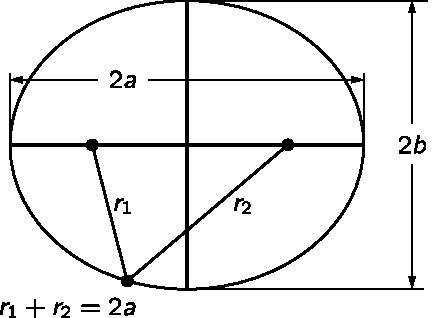
\includegraphics[width=0.25\textwidth]{Chapter7/椭圆}
    \caption{椭圆}
    \label{figure:椭圆}
\end{wrapfigure}
其次开普勒发现,行星并不以均匀速率绕太阳转动,而是当它们接近太阳时跑得较快,远离太阳时则跑得较慢,确切地说便是这样:设在任意相继的两个时间,比如说相隔为一周的时间内观察一个行星,并且对每个观察位置向行星画一条矢径\footnote{矢径是从太阳到行星轨道上任何一点的连线。}。那么行星在一周中所经过的轨道上一段弧线和两条矢径一起围成一定的平面面积,如图7.2所示的那个阴影面积。如果在离太阳较远的那部分轨道上(此时行星运动得较慢),也作时间相隔一周的与前类似的两次观察,那么这时围成的面积与前一情况下的面积完全相等。因此,按照开普勒第二定律,每个行星的轨道速率都使矢径在相等的时间内“扫过”相等的面积。

\begin{wrapfigure}{l}{0.3\textwidth}
    \centering
    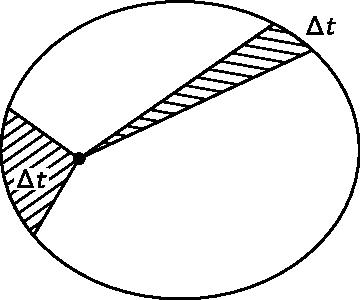
\includegraphics[width=0.25\textwidth]{Chapter7/开普勒的面积定律}
    \caption{开普勒的面积定律}
    \label{figure:开普勒的面积定律}
\end{wrapfigure}
开普勒第三定律发现得较晚,这条定律与前两条不同,各属于不同的范畴,因为它不是只涉及单独的行星,而涉及一个行星与其他行星之间的关系。这条定律表明:如果把任何两个行星的轨道周期和轨道大小进行比较,则周期与轨道大小的3/2次方成正比。这里所说的周期是行星在其轨道上完全绕一圈所需的时间间隔,而所谓轨道的大小使用椭圆轨道最大直径(术语叫“长轴”)的长度来量度的。更简单一些,如果行星绕圆周运动(实际上,它们也近于这样做),那么绕圆周走一圈所需的时间将正比于直径(或半径)的3/2次方。这样,开普勒三条定律便是:
\begin{enumerate}
\item[Ⅰ] 每个行星都沿椭圆轨道绕太阳运行,太阳位于各椭圆的其中一个焦点上。
\item[Ⅱ] 从太阳画到行星的矢径,在相等时间间隔内扫过相等的面积。
\item[Ⅲ] 任何两个行星的周期平方正比于它们各自轨道半长轴的立方:$T^2\sim a^2$。
\end{enumerate}


\section{动力学的发展}

当开普勒发现这些定律的时候,伽利略正在研究有关运动的定律。当时的问题在于什么东西使行星绕转运动(那时有一种理论这样说,行星之所以运行是因为在它们背后有看不到的天使在扑动它的飞翼,推动它们前进。你们将会看到,这个理论现在被修改了一下!这就是说,为了保持行星的绕转运动,看不见的天使必须朝与运动方向不同的方向飞行,并且它们也没有飞翼。除此之外,它倒多少有点像先前的理论!)在有关运动方面,伽利略发现了一个非常值得注意的事实,这个事实对于理解开普勒定律是必不可少的。这就是\uwave{惯性}原理——如果有某个物体在运动,但没有和其他东西相碰撞,也完全不受干扰,那么它将沿一直线以均匀速度永远运动下去。(\uwave{为什么}它能保持直线运动?我们不知道,但是事情就是如此。)

牛顿使这个观念更为明确,他说:“改变物体运动的唯一方法是要对之用\uwave{力}。”如果物体的速率变大,这必定有一个力施加在\uwave{运动方向上}。另一方面,如果物体的运动改变到另一个新的方向,那么它必定受到一个\uwave{斜向}的力作用。这样牛顿添进了如下一个概念:要改变一个物体运动的速率\uwave{或方向},就需要有力才行。例如:把一块石子系在绳上,使它旋转而作圆周运动,那么就需要有一个力以保持它在圆周上运行。这时我们必须把绳子\uwave{拉}住。事实上,这个定律说的是,力所产生的加速度反比于物体的质量;或者说,力正比于质量乘加速度。物体的质量越大,使它产生某一给定加速度所需的力就越大。(质量可以这样来测量,使其他石子系于同一根绳的末端,使它们以同样的速率绕同样的圆周转动,用这种方法可以知道它们所需的力的大小,质量较大的物体,所需的力较大。)从这些考虑中得出的一个卓越的观念就是:要保持行星在它的轨道上运行,根本不需要有一个\uwave{切向的力}(天使并不一定要沿切线方向飞行),因为行星总会沿所要求的方向运动,如果根本没有什么东西去干扰它,那么行星就将沿\uwave{直线}运行下去。但实际的运动却偏离了不存在力作用时物体所应沿之运动的那条直线,这种偏差差不多与运动相垂直,而不沿运动的方向。换句话说,由惯性原理得知,控制行星绕太阳运动所需的力不是一个\uwave{绕}太阳而是\uwave{指向}太阳的力。(如果有一个力指向太阳,那么当然太阳也许就是那天使了!)


\section{牛顿引力定律}

牛顿从他对运动定律的深入理解,意识到\uwave{太阳}可能是支配行星运动的那些力之渊源或机构所在,他给自己证明(或许我们不久也能证明),正是在等时间内扫过相等面积的这个事实,为所有偏离都是径向的这件事树立了一个明确的标志——也就是证明了面积定律是所有的力都精确地\uwave{指向太阳}这一观点的一个直接结果。

其次,对开普勒第三定律的分析可以表明,行星越远,作用力越弱。如果比较两个离太阳距离不同的行星,那么分析表明,力与行星各自的距离平方成反比。把这两条定律结合起来,牛顿于是推断说,必定存在着一个力,它的大小反比于两个物体间距离的平方,方向则沿着它们间的连线。

作为一个对事物普遍性有非凡触觉的人,牛顿当然要做出这种假设,认为这个关系可以更普遍地加以应用,而不只是限于太阳拉住行星这个事实。例如当时已经知道,正像月球绕着地球转动一样,木星也有自己的月球在绕着它转动,于是牛顿确信,每个行星都在用一个力拉住自己的月球。关于把\uwave{我们}吸住在地面上的那个力,牛顿也早已知道,所以,他就提出,这类力是一个\uwave{普遍存在}的力—— \uwave{每个物体都吸引任何其他一个物体}。

其次一个问题是,地球拉住人的力与它拉住月球的力是否“相同”,也就是说,是否都与距离平方成反比。如果地面上一个物体原来静止,然后释放,在第一秒内落下4.9米,那么在同样时间内,月球将落下多远?我们也许会说,月球根本没有落下。但是如果没有力作用在月球上,它会沿一直线离去,可是,它并不这样做而是沿一圆周运动,所以实际上它是从那个如果根本没有力作用时所应处的位置上\uwave{落}下来。从月球的轨道半径(约240,000英里)以及它绕地球一圈所需的时间(约为29天),可以算出月球在其轨道上每秒走了多远,随后就可以算出它在一秒钟内落下了多远\footnote{这就是说,月球的圆形轨道处在一根直线之下有多远,而这根直线就是对月球在一秒钟前在轨道上所处的那一点作的切线。}。经过计算这段距离约为$1/20$英寸。它与反平方定律吻合得非常好,因为地球的半径是4000英里,而如果,一个离地球中心4000英里的物体在第一秒内落下16英尺,那么一个在240,000英里,也就是在60倍远的地方的物体应当只掉下16英尺的$1/3600$,这个数值大约也为$1/20$英寸。为了想用类似的计算来检验这个引力理论,牛顿非常仔细地进行了他的计算,但是却发现差异很大,以至他认为这个理论与事实相矛盾,因为没有发表他的结果。六年之后,一个对地球大小的新的测量表明,天文学家曾使用了一个不正确的到月球的距离。当牛顿听到这个消息后,他就用正确的数据重新作了计算,所得的结果与事实非常一致。

\begin{wrapfigure}{r}{0.4\textwidth}
    \centering
    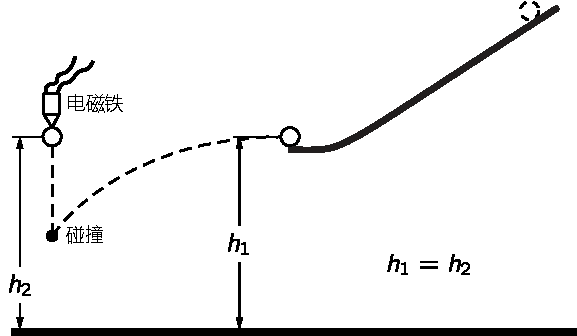
\includegraphics[width=0.35\textwidth]{Chapter7/演示垂直和水平运动互不相关的仪器装置}
    \caption{\footnotesize 演示垂直和水平运动互不相关的仪器装置}
    \label{figure:演示垂直和水平运动互不相关的仪器装置}
\end{wrapfigure}
月球“下落”的这种观念,多少有点使人迷惑,因为正像你们所知道的那样,月球丝毫没有靠近地球。但是这个观念相当有意思,以致值得进一步加以说明:所谓月球下落,其含义就是:它离开了不存在力的作用时原应遵循的那条直线。让我们举地球表面上的一个例子,一个靠近地面的物体被释放后,在第一秒内将降落16英尺,一个水平射出的物体也将降落16英尺;即使它沿水平方向运动,但在同样时间内它仍然要落下16英尺。图\ref{figure:演示垂直和水平运动互不相关的仪器装置}表示一个用以演示这一情况的仪器装置。

在轨道的水平部分有一个小球,它行将往前冲出一小段距离。在同一高度则有一个行将垂直下落的小球,另外,有一电动开关起控制作用,在第一个小球离开轨道的时刻,它随即释放另一个小球。至于两个小球在同样时间内落下同样的高度可以用它们在半空中相碰撞这个事实来证明。一个物体如子弹被水平射出时,可能在一秒钟内要跑很长一段路程——比如说2000英尺——但即使它是水平瞄准的,它仍然要落下16英尺。然而,如果我们把子弹发射得越来越快,那么会发生什么情况呢?不要忘记,地球的表面是弯曲的,如果子弹发射得足够快,那么在落下16英尺后,它可能恰巧在地面之上与之前相同的高度的地方。怎么会这样呢?子弹仍然在下落,但是由于地球向下弯曲,所以在“绕着”地球下落。问题是,它在一秒钟内必须跑多远才能使地球在水平线下面16英尺?在图7.4中,我们看到一个半径为4000英里的地球,以及一条在没有力作用的情况下子弹将循之而行的切向指向。
\begin{wrapfigure}{r}{0.35\textwidth}
    \centering
    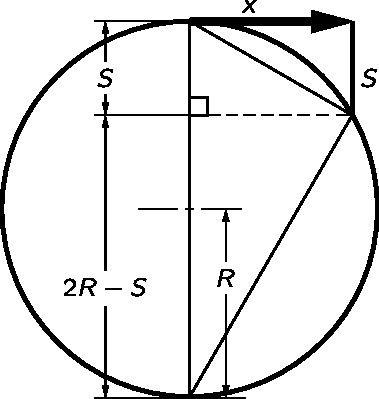
\includegraphics[width=0.3\textwidth]{Chapter7/指向圆形轨道中心的加速运动}
    \caption{\footnotesize 指向圆形轨道中心的加速运动。根据平面几何,$x/S=(2R-S)/x\approx 2R/x$,其中$R$是地球的半径(4000英里),$x$是每秒“水平通过”的距离;$S$是每秒“下落”的距离(16英尺)}
    \label{figure:指向圆形轨道中心的加速运动}
\end{wrapfigure}
如果我们现在应用几何学中一条奇妙的定理,即垂直于直径的半弦是所分割的直径两部分的比例中项,那么就可以看出,子弹所走的水平距离是所下落的距离16英尺与地球直径8000英里的比例中项。$(16/5280) \times 8000$的平方根很接近于5英里。于是我们看到,如果子弹每秒跑5英里时,那么它将继续以同样的速度每秒往地球落下16英尺,而决不会与之靠得更近一些,因为地球总是在不断地弯曲而离开子弹。加加林先生也是这样以每秒大约5英里的速率绕地球飞行25000英里来使自己保持在太空中的(他绕地球一周所需的时间稍微长一些,因为他在稍微高一点的地方飞行。)

只有在所获得的超过所给予的时,任何一个新定律的重大发现才有价值。现在,牛顿\uwave{用}开普勒第二和第三定律来推导他的引力定律,那么他都有那些\uwave{预言}?首先,他分析了月球的运动,因为他把地面上物体的下落与月球的下落联系起来了。接下来问题是它的\uwave{轨道是椭圆吗}?我们在往后的一章中将看到如何能精确地计算这个运动,而且人们确实能够证明,它的轨道应当是一个椭圆\footnote{这在本教程将不予证明。},所以毋需再用其他事实来说明开普勒\uwave{第一}定律,这样,牛顿作出了他第一个有力的预言。

引力定律解释了很多之前不能理解的现象。例如,月球对地球的吸引造成了潮汐,这在当时还是一个迷。月球把它下面的水吸引上来造成潮汐——这在以前人们也想到过,但是他们不如牛顿那样聪明,所以他们想一昼夜应该只有一次潮汐。其理由是,月亮把下面的水吸引上来,造成一个高潮和一个低潮。由于地球在月球下面旋转,就使一个地方的潮水每24小时涨落一次。实际情况是潮水每12小时涨落一次。另一个学派则主张,高潮应当在地球的另一面,他们争辩说,因为月球把地球从水中拉开!这两种理论都是错误的。实际的过程如下:月球对地球和对水的吸引在中心是“平衡”的,但是靠近月球的水被拉的程度要比平均值\uwave{大},而离月球较远的水被拉的程度要比平均值\uwave{小}。此外,水能流动,而比较结实和坚硬的地球却不能,真正的情况是这两种情况的结合。

\begin{wrapfigure}{r}{0.4\textwidth}
    \centering
    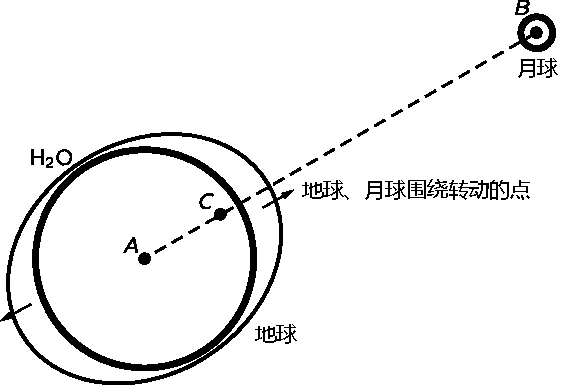
\includegraphics[width=0.35\textwidth]{Chapter7/解释潮汐现象的地球-月球系统}
    \caption{解释潮汐现象的地球-月球系统}
    \label{figure:解释潮汐现象的地球-月球系统}
\end{wrapfigure}
所谓“平衡”指的是什么意思呢?什么东西在平衡?如果月球把整个地球拉向自己,那么为什么地球不会“向上”落到月球上去?这是由于地球耍着像月球一样的花招,所以它在绕某点作圆周运动,这个点在地球内部,但不在地球中心。月球并不在绕地球转动,而是地球和月球一起在绕一个中心位置转动,每一个都在向着这个共同位置下落,如图7.5所示。这个绕共同中心的运动,是使每一个的下落得以平衡的原因。因此,地球也不是沿一直线行走,而是在绕一个圆周转动。地球上远的一边的水波是“不平衡的”,因为该处月球的引力要比在地球中心处小,而在地球中心处这一引力刚好和“离心力”平衡,结果这一不平衡使水沿离开地球中心的正方向运动。在近的一边,月球的吸引较强,所以不平衡是在空中相反的方向上,但又是\uwave{离开}地球的中心。最后,我们得到\uwave{两次}潮汐。



\section{万有引力}

当我们理解引力的时候,还可以理解别的什么呢?人人都知道地球是圆的。为什么地球是圆的?这很容易回答:由于引力的作用。我们之所以能够理解地球是圆的,仅仅是因为每个物体都在吸引任何其他的物体,所以地球尽它之所能把自身各部分相互吸引在一块!如果我们进一步深入下去,那么地球并非是一个\uwave{精确}的圆球,因为它在旋转着,从而引进了离心效应,在靠近赤道的地方,它趋向于与引力相对抗。其结果表明,地球应当是椭圆形的,而且我们甚至得到了这个椭圆的正确形状。这样,我们仅仅从引力定律出发,就能推论出太阳,月球和地球都应当是(近似的)圆球形。

应用引力定律我们还能做别的什么呢?如果我们看一下木星的月球,那么我们就能知道它们怎样围绕这个行星运行的一切情况。附带说一下,在有关木星的月球这个问题上曾经出现过一个困难,值得在这里一提。罗末(Roemer)非常仔细地研究了这些月球,他注意到,它们时而好像走在时间表的前面,时而好像走在时间表的后面。(等待很长一段时间,并找出这些月球绕行一圈平均所需的时间,就能找到它们的时间表。)当木星特别\uwave{靠近}地球时,它们走在前面,而当木星\uwave{远离}地球时,它们就走在\uwave{后面}。因而要按照引力定律来解释,看来这是一件非常困难的事——确实,如果找不到其他解释的话,这就会成为这个奇妙理论的终结。如果某条定律,只要在\uwave{一个}理应起作用的地方不起作用,那它\uwave{就是}错的。但是现在出现这个矛盾的原因是十分简单和美妙的:为了\uwave{看到}木星的月球就需要稍微花一点时间,因为光从木星跑到地球上来是需要时间的。当木星靠近地球时,它花的时间稍微少一点,而当木星远离地球时,所花的时间就稍微长一点。这就是为什么这些月球平均而论好像时而超前、时而稍微落后的原因,完全看它们靠近还是远离地球而定。这个现像表明光的传播并不是在一瞬间发生的,并且它第一次为光的速度提供了一个估计值,这个估计值是在1676\footnote{原文为1656,经查证为1676。——译者注}年做的。

\begin{wrapfigure}{r}{0.4\textwidth}
    \centering
    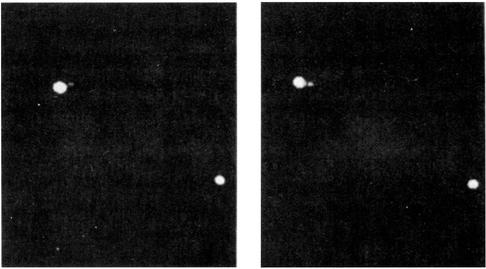
\includegraphics[width=0.35\textwidth]{Chapter7/双星系统}
    \caption{双星系统}
    \label{figure:双星系统}
\end{wrapfigure}
如果所有的行星彼此之间都相互吸引,那么控制一个行星比如说木星围绕太阳转动的力,不是只有从太阳来的引力,也有来自土星的拉力。实际上这个力并不强,因为太阳的质量比土星要大得多,但是毕竟有一点吸引作用,所以木星的轨道不应该是一个精确的椭圆,事实也确实是这样。它与正确的椭圆轨道稍有偏离,而且绕着它“摆动”。这样的运动就有点复杂了。人们曾视图在引力定律的基础上分析木星、土星及天王星的运动。对这些行星中的每一个,人们计算了它对其他行星所产生的效应,以便知道这些运动中出现的微小偏差与不规则性,是否单独用\uwave{这条}定律就能完全理解。好,就让我们看一下吧!对于木星和土星,一切都很好,但是对天王星却是“不可思议”的,它以非常奇特的方式运行着。至于它不是沿着一个精确的椭圆运行,那是可以理解的,因为有木星和土星在吸引它。但是,即使考虑到这些引力,天王星\uwave{仍然}没有按正确方式运行,所以引力定律就面临被推翻的危险,这是一个不能排除的可能性。但在英国与法国有两个人,亚当斯(Adams)与勒维耶(Le Verrier),他们各自设想了另一种可能性,或许存在着\uwave{另一个}幽暗而看不见的行星,以致人们从未看到过它,这个行星$N$可能在吸引天王星。他们计算了这样一个行星应处在那个位置才能造成所观察到的那个扰动。他们把这一消息分别通知有关的天文台,并说:“先生们,把你们的望远镜指向某某、某某位置,你们就会看到一颗新的行星。”至于人们对你注意不注意,那常常要看你在同谁进行联系。他们确实注意到了勒维耶;他们朝那个位置看了,果真发现有一颗行星$N$!另一个天文台过了几天也很快地看到了这颗新行星。

这个发现表明,牛顿定律在太阳系范围内是绝对正确的;但是这些定律能够扩展到离我们最近的相对距离较小那几个行星之外吗?第一个检验是回答这个问题:\uwave{恒星}是否也像行星一样在\uwave{彼此吸引}?在双星的情况下,我们有确凿的证据表明,它们是在彼此吸引。图7.6表示一对双星——两颗非常靠近的恒星(图上还有第三颗恒星,由此我们看出照片没有被偏转)。

图中也显示了双星在几年之后所在的位置,我们看到,相对于“固定”的恒星来说,双星的轴转过了一定角度,也就是说两颗星中每一颗在绕着另一颗转动。它们是不是在按照牛顿定律转动?图7.7表明对这种双星系统中一颗星的相对位置所作的测量。

这里我们看到一个完美的椭圆,测量工作从1862年开始,到1904年测完了整个一圈(到现在为止它必定又已绕行一圈多了)。一切与牛顿定律相一致,只是天狼星A\uwave{不再焦点上},为什么是这样?因为椭圆平面并不在“天空平面”上。我们不是从垂直方向去看轨道平面,而当从倾斜方向去看时,它还是一个椭圆,但焦点不再在同一个位置上。因此我们确实能够按照引力定律的要求来分析双星中一个绕另一个的运动。

\begin{figure}[htbp]
    \centering
    \begin{minipage}[t]{0.4\textwidth}
        \centering
        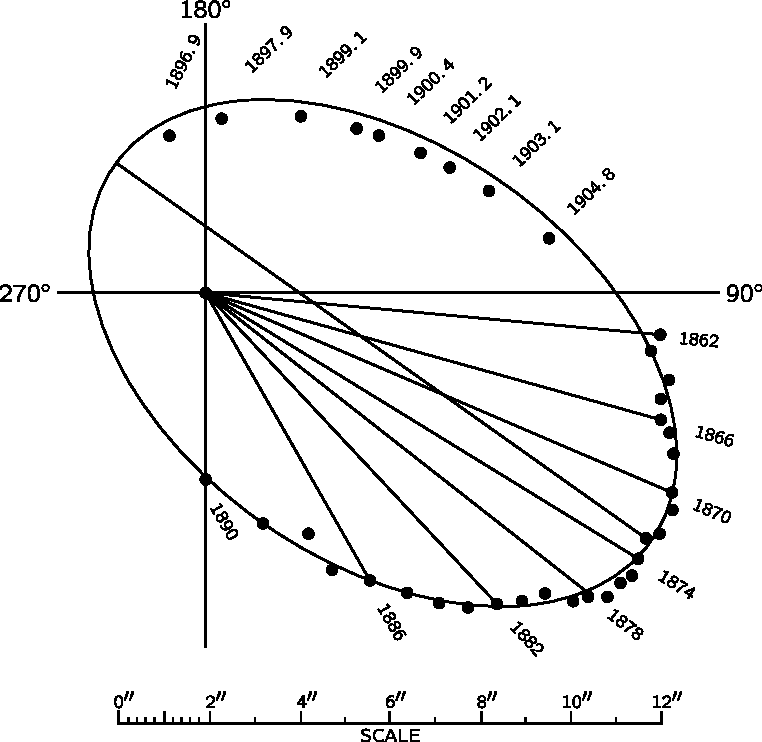
\includegraphics[width=5cm]{Chapter7/天狼星B绕天狼星A转动的轨道}
        \caption{天狼星B绕天狼星A转动的轨道}
        \label{figure:天狼星B绕天狼星A转动的轨道}
    \end{minipage}
    \begin{minipage}[t]{0.4\textwidth}
        \centering
        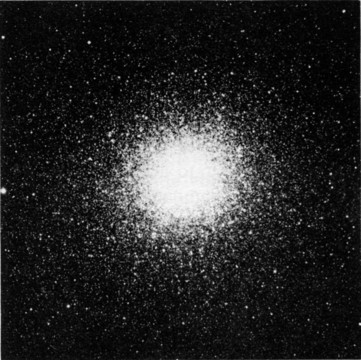
\includegraphics[width=5cm]{Chapter7/球状星团}    
        \caption{球状星团}
        \label{figure:球状星团}
    \end{minipage}
\end{figure}

\begin{figure}[htbp]
    \centering
    \begin{minipage}[t]{0.4\textwidth}
        \centering
        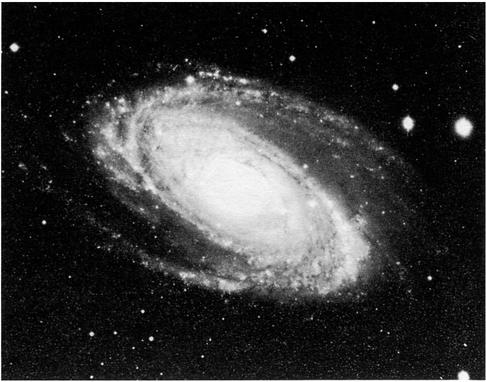
\includegraphics[width=5cm]{Chapter7/某星系}
        \caption{某星系}
        \label{figure:某星系}
    \end{minipage}
    \begin{minipage}[t]{0.4\textwidth}
        \centering
        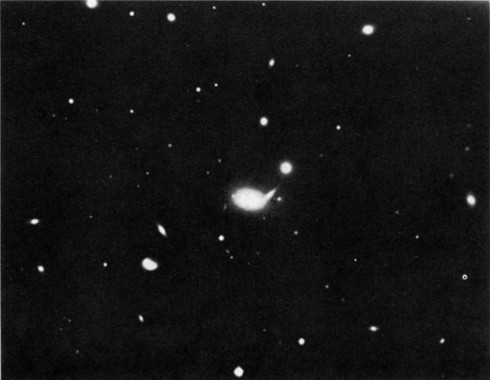
\includegraphics[width=5cm]{Chapter7/星系团}    
        \caption{星系团}
        \label{figure:星系团}
    \end{minipage}
\end{figure}

甚至对更大的距离引力定律也是正确的,图7.8表明了这一点。如果一个人看不出引力在这里起作用,那他过于迟钝了。这幅图所显示的是天空中最美妙的事物之一——一个球状星团。所有的小点都是星星。虽然看上去它们好像向中心密集地挤成一团,其实这是由于我们的仪器难免发生错误所致。事实上,即使是最靠近中心的那些恒星之间的距离也非常巨大,而且它们也非常难得相互碰撞。在内部比在外沿有更多的恒星,越往外走,恒星越少。很明显,在这些恒星之间存在着一个引力。因此非常清楚,在如此巨大的、或许是太阳系大小的100,000倍的范围内也存在着引力的作用。让我们现在跑得更远一点,看一下图7.9所示的\uwave{某一银河系}的整体。这个银河系的形状表明它的物质明显地有团聚在一起的趋势。当然我们不能证明这一定律在这里也是准确地与平方成反比,而只能说明在如此巨大的范围内,仍然有一个引力作用着,它把整个物体聚集在一起。有人或许会说:“嗯,这一切真是太奇妙了,但是为什么不聚集成一个球呢?”回答是:因为它在\uwave{旋转},并且具有\uwave{角动量},而这是在它收缩时所不能放弃的;因此,它必然主要在一个平面内收缩(附带提一下,如果你想寻找一个合适的问题,那么银河系的旋臂如何形成,以及究竟是什么决定了这些银河系的形状等等,都还没有进行研究。)然而,非常清楚,银河系的形状来源于引力的作用,尽管它的结构的复杂性还不允许我们把它完全分析清楚。一个银河系的规模大约有50,000到100,000光年,地球到太阳的距离是$8\frac{1}{3}$光\uwave{分},所以你们可以看到这样的范围是多么的大!

正如图7.10所指出的那样,甚至在更大的范围内也存在着引力。图中还显示出有许多“小”的东西集成一簇,这就是一个犹如星团一样的\uwave{银河系团}。可见这些银河系相距如此之大也彼此吸引而同样聚集成团。或许甚至在超过\uwave{几千万}光年的距离之间也存在着引力作用,就我们今天所知,看来引力永远以与距离的平方成反比的方式延伸出去。

\begin{figure}[htbp]
    \centering
    \begin{minipage}[t]{0.4\textwidth}
        \centering
        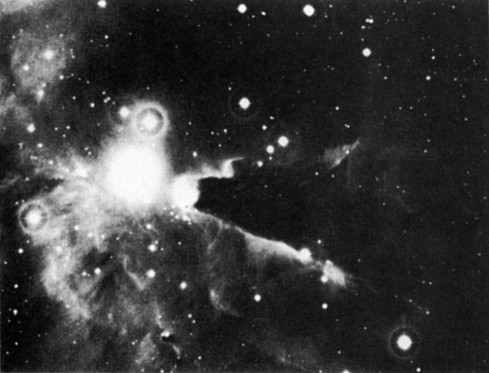
\includegraphics[width=5cm]{Chapter7/星际尘埃云}
        \caption{星际尘埃云}
        \label{figure:星际尘埃云}
    \end{minipage}
    \begin{minipage}[t]{0.4\textwidth}
        \centering
        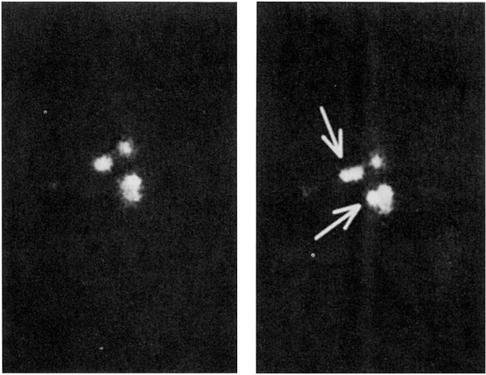
\includegraphics[width=5cm]{Chapter7/新星的形成}    
        \caption{新星的形成}
        \label{figure:新星的形成}
    \end{minipage}
\end{figure}


我们不仅能够理解星云,而且从引力定律出发,甚至还能对恒星的起源获得某些概念。如果我们有很大的一片尘埃与气体云,如图7.11所示,那么尘埃片与片之间由引力而产生的吸引,可能会使它们形成一些小的团块。在图上有一些“小”黑斑依稀可辨,它们可能是尘埃与气体相积聚的开始,而由于这些积聚物彼此间的引力作用,就开始形成星体。我们究竟是否看到过一个星的形成,这是一个可争论的问题。图7.12提供了一个证据说明我们曾经见到过。左边是一张1947年拍摄的照片,显示一个气体区域,中间有几个星体;右边是一张只过了7年之后拍摄的照片,显示两个新的亮点。气体是不是积聚了起来,引力是不是作用得足够强,并把它聚集成一个足够大的球体,以致在其内部发生星体核反应而把它变为一颗星呢?或许是这样,或许不是这样,而不近情理的是,仅仅在7年之中我们竟会如此幸运,能看到一颗星把本身转变为可见的形式;更不可能的是,我们居然一下子能看到两个!

\section{卡文迪什实验}

由前所见,引力作用伸展到距离极大的地方。但是,如果在\uwave{任何}一对物体之间有一个力作用着,那么我们应当能够测出作用在我们周围物体之间的这个力。比方说,难道不能用一个铅球和一个大理石球来做实验,观察大理石球朝向铅球跑去,而一定要去观察星体的相互绕行吗?用这样一种简单方式来做这个实验,其困难在于,这里的力是非常之弱的。因此必须格外小心地来对待,这就是说,要把仪器遮盖起来以避免与空气接触、要肯定它不带电等等;然后可以来测量这个力。卡文迪什(Cavendish)第一个进行了这种测量,他所使用的仪器的略图如图7.13所示。

\begin{wrapfigure}{r}{0.4\textwidth}
    \centering
    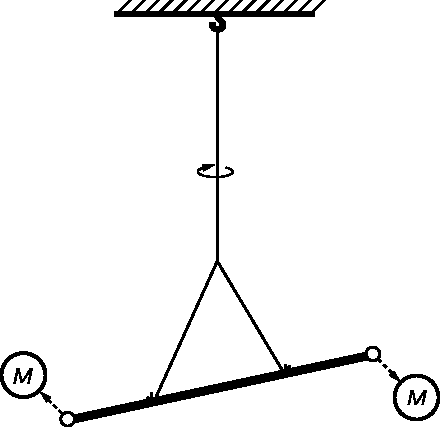
\includegraphics[width=0.35\textwidth]{Chapter7/卡文迪什测量引力常数的装置}
    \caption{卡文迪什用来验证小的物体之间存在万有引力和测量引力常数$G$的装置略图}
    \label{figure:卡文迪什测量引力常数的装置}
\end{wrapfigure}
这个实验第一次演示了两个大的固定铅球和两个小铅球之间力的直接作用;两个小铅球装在一根细杆的两端,细杆用一根非常精细的、称为扭丝的金属丝悬挂起来。用测量扭丝扭转了多少的方法,我们就能测出力的强度,证实它与距离平方成反比,并确定它的大小。这样,我们就能精确地确定公式
\begin{equation*}
F=G\,\frac{mm'}{r^2}.
\end{equation*}
中的系数$G$,因为质量和距离都是已知的。你们会说,“对地球来说我们早就知道这个系数了。”是的,但我们并不知道地球的\uwave{质量}。如果从这个实验知道了$G$,以及地球的吸引有多强,我们就能间接地知道地球的质量有多大!这个实验曾经叫做“称地球”实验。卡文迪什也声言他称了地球,但是他实际测量的是引力定律的系数$G$。这是唯一能确定地球质量的方法。$G$的数值是
\begin{equation*}
6.670\times10^{-11}\text{牛顿}\cdot\text{米}^2/\text{千克}^2.
\end{equation*}

引力理论的这一伟大成就在科学史上所产生的重大影响,怎么估计也不会过分。请把早先年代里无休止的争论和悖论盛行,知识中充满着混乱、迷惑以及不完善和不可靠这种情况同这条定律的明晰和简单做个比较吧!——现在,所有月球、行星和恒星都由这样一条\uwave{简单的规则}来支配,并且,人们能够理解它,从它推论出行星应当如何运动!这是科学在以后年代里所以会获得如此巨大成就的原因,因为它为人类理解宇宙间其他现像提供了一个希望,可能也有这样一种特别简单的定律来支配它们。


\section{什么是引力}

然而这条定律确实是如此简单吗?什么是它的机制?我们所做过的一切,不过是描写了地球\uwave{怎样}绕太阳运行,但是我们没有谈到是\uwave{什么东西在使它运动}。牛顿对此没有做过任何假设;他满足于找出它做的是\uwave{什么},而并不深入到它的机制中去。从那时起也没有人提出过任何机制。物理定律的特征,就是它们具有这种抽象的性质。能量守恒定律是一条关于这样一些量的定理,对于这些量必须加以计算,然后把它们加起来,但它没有提到它的机制;同样,力学的那些重要定律也是一些数学定律,我们并不知道起作用的机制是什么。为什么我们能用数学来描述自然,而在其背后有没有一个机制呢?无人知道。我们必须继续照此办理,因为用这种方法我们能够发现更多的东西。

引力的机制曾经屡次为人们所提到过,研究了一下很多人一再想到的其中的一个,是颇有趣味的。起初,当有人“发现”它的时候,确实非常高兴,感到十分幸运,但他随即发现原来这是错误的。这个机制大约在1750年第一次被人们提出。设想有许许多多粒子在空间以极大速度向各个方向运动,在它们穿过物质时只有很少一部分被吸收掉,当它们被吸收时,就给地球以一个冲量。然而,由于在一个方向上运动的粒子同在别的方向上运动的粒子一样多,所以这些冲量都互相抵消。但是来自太阳的粒子比来自另一边的粒子要少一些。因此,地球最后受到一个朝向太阳的冲量,而且,不要花费多少时间人们就能看出,这个冲量与距离的平方成反比,因为当距离改变时,太阳所张的立体角也要改变。这个机制错在那里呢?错在其中包括了一些新的结果,而这些新的结果是不\uwave{真实}的。这个特别的想法遇到了如下困难:地球绕太阳运行时,它与从前面射来的粒子相碰撞的次数,将比从后面射来的粒子要多。(当你在雨中奔跑时,打在你脸上的雨点要比打在你脑后的多!)因此从前面将给予地球更大的冲量力,而地球将会受到一种\uwave{对其运动的阻力作用},这种阻力使它在轨道上的运动减慢下来。人们可以算出,作为这种阻力的结果,地球需要多长时间才会停下来,结果是地球仍留在轨道上的时间并不长,所以这个机制行不通。从此也就没有再提出过任何一个机制,它既能“解释”引力,又不致于会预言其他实际\uwave{不}存在的现像。

其次我们要讨论万有引力与其他作用力之间可能存在的关系。目前还没有一种用其他力来说明引力的解释。它不是电或诸如此类的一个方面,所以我们无法解释。然而,引力和其他力十分相似,因而看一下它们的相似之处是很有趣的。例如,两个带电体之间的电力看上去就很像引力定律:它们之间的电力等于一个带负号的常数乘以电荷之积,并与距离的平方成反比。电力的方向则与引力的情况相反——同号相斥。但是两条定律含有同样的距离函数,这难道还不够引人注目?引力与电力之间的关系或许比我们所能想像的要密切得多。人们做了许多尝试试图把它们统一起来;所谓的统一场论不过是一个想把电力和引力结合起来的非常美妙的尝试而已;但是如果把引力与电力相比较,那么最有趣的事是力的\uwave{相对强度}。任何一个包括它们两者的理论,必须也能推导出引力有多大。

如果我们来看用某些自然单位表示的由于电作用产生的两个电子(自然界中的电荷的基本单位)之间的斥力,以及两个电子由于它们的质量而产生的引力,那么我们就能求出电斥力与万有引力的比值。这个比值与距离无关,是自然界的一个基本常数,如图7.14所示。两个电子间的万有引力与电斥力之比等于1比 \num{4.17d42} !现在的问题是,这样巨大的数字从何而来?正像地球与跳蚤的体积之比那样,这个数值不是偶然的。这个大得难以置信的数字是一个自然常数,所以它包含了自然界中某种深邃的性质。这样一个惊人的数字从哪里来呢?有些人说,总有一天我们会找到一个“宇宙方程”,其中的一个根就是这个数。要找到这样的方程,它确能以大得如此出奇的数字为一个自然根,那是非常困难的。人们也曾想到过其他的可能性;其中之一是把它与宇宙年龄联系起来。很清楚,我们必须在某个地方找到\uwave{另一个}巨大的数字。那么,我们是不是用\uwave{年}来表示宇宙的年龄呢?不,因为年不是“自然”量;它只是人们所想像出来的。作为某种自然量的一个例子,让我们来看一下光穿过一个质子的时间,它是 \numb{d-24}秒。如果我们把这个时间与 \uwave{宇宙年龄} \numb{2d10}年相比较,那么答案是 \numb{d-42}。它有大约相同数目的零跟在后面,因而有人提出,引力常数与宇宙年龄有关。如果情况真是如此,引力常数就会随时间而变化,因为随着宇宙的变老,宇宙年龄与光穿过一个质子所需的时间之比就会逐渐变大。

那么,引力常数是否可能随着时间\uwave{在}发生变化呢?当然,这种变化如此之小,以致要确定它是相当困难的。

\begin{wrapfigure}{r}{0.4\textwidth}
    \centering
    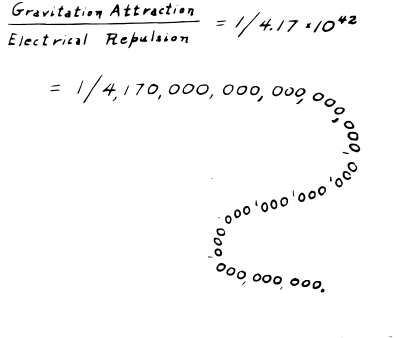
\includegraphics[width=0.35\textwidth]{Chapter7/两个电子之间的电力相互作用和引力相互作用的相对强度}
    \caption{两个电子之间的电力相互作用和引力相互作用的相对强度}
    \label{figure:两个电子之间的电力相互作用和引力相互作用的相对强度}
\end{wrapfigure}
这里我们能够想到的一个检验方法是确定在过去 \numb{d9} 年中这种变化可能产生过什么影响。\numb{d9}年大约是地球上出现最早的生命以来到目前为止的时间,是宇宙年龄的十分之一,在这段时间内,引力常数可能增加大约百分之三十,从这里可以得出,如果我们考虑到太阳的结构——即太阳物质的重量与其内部产生辐射能的快慢的平衡,那么我们可以推论说,如果引力增加百分之十,则太阳的亮度要增加比百分之十大得多——即引力常数的\uwave{六次方}。如果我们计算一下,引力改变时地球轨道会发生什么情况,那么我们将发现,地球那时已更\uwave{靠近}太阳。总而言之,地球将变得更热(大约摄氏100度),所有的水不会再留在海洋里而变成了充满在空气中的水蒸汽,这样,生命也就不会从海洋里开始。所以我们现在并\uwave{不}相信,引力常数是随着宇宙的年龄而改变的。但是,这样一些论证像我们刚才所给出的那样,是不会十分令人信服的,这个问题还没有完全得到解决。

众所周知,物体的重量正比于它的质量,而这种质量实质上就是惯性的一种量度,也就是当一个物体作绕圆周运动时,要维持它在圆周上有多难的一种量度。因此,若有一轻一重两个物体,由于重力作用而绕一更大的物体沿同一个圆周以同样速度转动,那么它们总将保持在一起,因为要在圆周上运动就\uwave{需要}力,对大的质量,需要的力也大。这就是说:对于一个较重的物体,重力作用应当\uwave{正好以恰当的比例}增加,所以这两个物体仍将一起做圆周运动。如果一个物体原先在另一物体的里边,那么它将\uwave{留在}里边而不离开;这是一个完全的平衡状态。因此,加加林或季托夫发现宇宙飞船舱内的一切东西是“失重”的,比方说如果他们碰巧丢掉一支粉笔,那么粉笔将与整个宇宙飞船沿着一条完全一样的路径绕地球飞行,所以它将始终在空间悬浮于宇航员的眼前。非常有趣的是,重力以极大的精密度\uwave{精确地}与质量成正比,因为如果不是如此的话,将产生某种效应,其中惯性与重量会有所区别。这样一种效应实际上并不存在。关于这一点,人们曾以极大的精密度用实验验证过,厄缶(fǒu)(E\"otv\"os)在1909年第一次进行了这种实验,而最近则由迪凯(Dicke)做过。对于所有做过实验的物质,它们的质量和重量的正比关系精确到了十的九次方之一或者更小,这真是个了不起的实验啊。



\section{引力和相对论}

另一个值得讨论的论题是爱因斯坦对牛顿引力定律所作的修正。尽管牛顿引力定律创造了所有这些惊人的成就,但仍然是不正确的!爱因斯坦对它所作的修正,在于把相对论考虑了进去。依照牛顿的观点,引力效应是瞬时发生地,也就是说,如果我们移动一个物体,那么我们就会立即感觉到一个新的力,因为物体到达了新的位置;按照这种说法,我们可以以无穷大的速度发送信号。然而爱因斯坦提出了种种论证,说明我们不能发送比光更快的信号,所以牛顿引力定律必定是错误的。在考虑到延迟情况而加以校正后,我们得到一条新的定律,称为爱因斯坦引力定律。这条非常容易理解的新定律的一个特点是:在爱因斯坦相对论中,任何具有\uwave{能量}的东西也具有质量——质量应在这一意义下来理解,即它以引力方式被其他质量所吸引。即使是光,由于它有能量,也就是有“质量”。当一束带有能量的光经过太阳附近时,它将受到太阳的吸引。所以光并不是沿直线行进的,而是被弯曲了的。例如在日食时,太阳周围的恒星应该看起来好像从它们的那些位置偏离出去了,这些位置就是如果太阳不在那里它们所应处的地方。而人们也观察到了这个情况。

最后,让我们把引力理论与其他理论比较一下。近年来我们发现,所有物质都由微小粒子所构成,并且世界上存在着几种相互作用,如核力等等。但是在这些核力或电力中还没有发现有那一个能用来说明引力。大自然的另一方面量子力学还没推广到万有引力。当尺度小到需要考虑量子效应时,引力效应是如此的微弱以至于根本没有必要发展一种有关万有引力的量子理论。另一方面,为了物理理论的内在一致性,重要的一点是看看是否牛顿定律修正为爱因斯坦定律之后,还可不可以进一步加以修正,使之与测不准原理相协调。到目前为止还没有完成这最后的修正。
